\chapter{Introduction}
\label{introduction}

Bicycle riding is a fundamental part of everyday transportation in many countries around the world. Ever since the development of the safety bicycle(two equal sized wheels, pneumatic tires, chain drive, rear wheel propulsion and a bent front fork), almost 130 years ago, the bicycle remains  one of the most prominent means of transport \cite{kooijman2013review}. With the growing concerns of sedentary lifestyles many choose the bicycle as their primary commute vehicle with the hopes of maintaining some levels of fitness. Additionally the bicycle is the preferred means of physical exercise for the elderly especially in the Netherlands and Denmark. Despite the fact that riding a bicycle is an acquired skill that we learn from our early childhood and we use throughout our life, the fundamental laws of human bicycle control are not yet understood.
\par

According to the European Road Safety Observatory \cite{eu2018cycle} in 2016 about 2.000 cyclists
were killed in road accidents throughout the EU. Despite the overall reduction in the road toll (down 40\% from 2007), the proportion of cycling related fatalities increased, from 6\% in 2007 to 8\% in 2016 \cite{eu2018cycle}. In a recent study examining the entries of patients to the emergency department due to traffic related accidents in the Netherlands (see Fig. \ref{fig:figure1}), it was found that cycling accidents were the most prevalent. With over 60,000 reported cases  bicycle accidents outnumber automobile accidents more than 4 to 1. It therefore  becomes clear that a lot could be done to improve cycling safety. Further look at the figure will reveal that most of those accidents did not involve a second party. In these cases the rider just fell off his bike. Although there are several potential reasons that riders lose control of the bicycle, formulating a general model of  how humans control single track vehicles could prove invaluable in understanding the causes behind the above numbers.

\begin{figure}[ht]
    \centering
    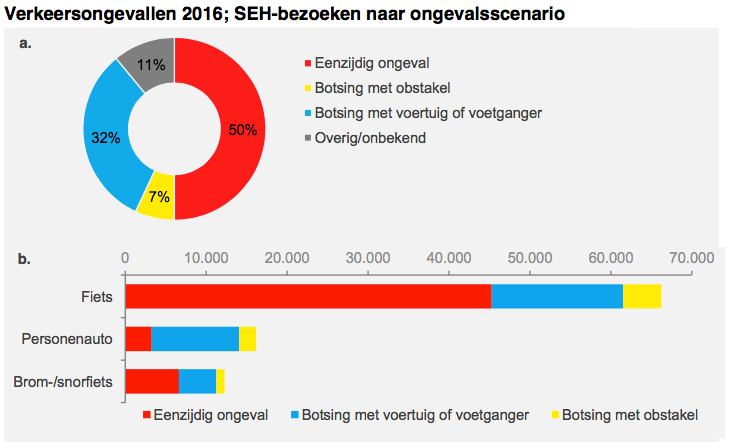
\includegraphics[scale=0.8]{images/figure1_1.png}
    \caption[Short title]{The number of road users that visit the emergency department at a hospital after a traffic accident in the Netherlands in 2016. Red indicates single vehicle accidents, yellow indicates a collision with an obstacle, blue indicates multi-vehicle accident and grey indicates other type of accidents\cite{krul_nijman_stam_2016}.}
    \label{fig:figure1}
\end{figure}

Following the steps of early cybernetics research in which airplane pilot modeling was pioneered by McRuer\cite{mcruer1959human,mcruer1967manual,mcruer1967manual2}, a plethora of authors attempted adapting McRuers crossover model in order to model the rider of a seemingly much more complex task; motorcycle and bicycle riding. However, some argued that such an approach will not work since cycling is not just a compensatory task. Moreover little concern was made to the fact that humans try to optimize for performance while simultaneously exerting the lowest amount of control effort. These spawned a new wave of research focusing in optimal control.  This approach is based in early motor control research in which the human brain is believed to work as a constrained optimal controller. 

A further look in motor control research  reveals the importance of the internal model in control, state estimation and dead time compensation \cite{francis1976internal, garcia1982internal, wolpert1995internal, gillespie2016human}. The internal model  theory argues that the motor system is controlled by the constant interactions between the process and the controller. In this case the process is the body, however in tasks like cycling the bicycle can be considered as an extension of the body. The internal model can be used either as a tool for control in the form of the inverse model \cite{edelmann2015,getz1995internal} or as a forward model in state estimation in combination with Kalman filters \cite{wolpert1995internal}. Additionally, forward models can be used in delay compensation algorithms \cite{miall1993cerebellum,van2001adaptive}. 
\newpage
In this work an attempt to iterate over existing rider control models is made with the goal of answering two important questions. 
\begin{itemize}
        \item How significant is the effect of torque feedback for the balance task of bicycling?
        \item What is the prediction strategy best suitable for dead time  compensation in the balance task of bicycling?
\end{itemize}

In order to answer the above questions system identification techniques are employed using  the experimental dataset acquired within the scope of this thesis. In \cref{chapter2} an attempt is made to investigate the effect of haptic feedback in the task of balancing a bicycle under lateral perturbations. Non-parametric identification was conducted on the response of 20 riders in two different experimental conditions. In the first one the experimental bicycle operated as a normal bike while in the second the coupling between roll and steer was modified in order to cancel the torque feedback that would naturally transfer from the front wheel contact point to the handlebars. In \cref{hapticFB} further analysis is conducted by applying gray box identification techniques in order to investigate again the importance of torque feedback but also to test the effect of time delays in sensory feedback pathways and how these can be compensated through the use of internal model theory. In \cref{app:A,app:B,app:C} further details are presented on the methodology used to acquire proper measurements from the sensors of the experimental platform.


% Every human-machine system requires an understanding of how the plant operates. In the case of the bicycle multiple efforts have been made in capturing the dynamics of the bicycle and its  self-stabilizing behavior. These have resulted in a set of linearized equations of motion, now  commonly referred to as the Whipple Carvalho model \cite{meijaard2007linearized}, which is going to be discussed further in chapter \ref{results}.\par
% As it is known single track vehicles are not stable at low speeds. This is why a controller (like the human rider) is required to close the loop and create a stable system. There are two ways with which the human affects the dynamics of the plant. The first is with its passive interactions with the plant as a physical multibody system. Most passive models model the rider as a point mass rigidly attached to the rear frame, or as a pendulum connected to the rear frame \cite{eaton1975man}, although recent efforts have been made to extend this further with more complex passive rider models which include modeling of neuromuscular dynamics with spring-damper systems at various interfaces between rider and the bicycle frame\cite{dialynas2019}. The second is with its active control behavior. This involves the active control motion, such as steering, leaning or pedaling, applied by the rider to control and balance the bicycle. In most such cases, the passive behavior  of the rider is simplified by only  accounting for a fixed mass on the seat post, but when lean torque needs to be examined more complex modeling is required. The focus of the study is to explore the available models that best express the human rider as a controller in the bicycle-rider closed loop system.\par
% The literature review presented herein gives an overview of research done in the field of active rider modelling  concerning single-track vehicles, while discussing with which methods and to what extent have these models been validated. This extensive overview is given in section \ref{sub:rider} of chapter \ref{results}, which is structured in three sections: \ref{ch:classical} Classical control system design, \ref{ch:optimal} Optimal control system design and \ref{ch:other} Other control system design. Chapter \ref{conclusions} concludes on the results from Chapter \ref{results} having as a final goal to answer the research question:
% \par
% • \textbf{What is the controller that best simulates the behavior of the human in the control of single track vehicles?}

